\documentclass[12pt]{article}

\setlength{\parindent}{0pt}
\setlength{\parskip}{2mm}

\usepackage{geometry}
 \geometry{
 letterpaper, left=20mm, right=20mm,  top=20mm,
 }
\usepackage{graphicx}
\graphicspath{ {graphics/} }
\usepackage{amssymb}

%%%%%%%%%%%%%%%%%%%%%%%%%%%%%%%%%%%%%%%%%%%%%%%%%
\title{RFC 2 - Boolean Value Encoding in Transmission Protocol}
%%%%%%%%%%%%%%%%%%%%%%%%%%%%%%%%%%%%%%%%%%%%%%%%%

\author{
	Noah Strong
}

\date{\today\ -- v1.1}

\begin{document}

\maketitle

\tableofcontents{}

%%%%%%%%%%%%%%%%%%%%%%%%%%%%%%%%%%%%%%%%%%%%%%%%%
\newpage

\section{Introduction}

We would like to find a way to encode a binary value in each transmission
along with the UID.
The encoding must not interfere with our current collision detection work
and should not require a massive overhall of the transmission protocol as it
currently stands.

\section{Background}

Patrick has requested that we look into adding the ability for a transmitter to
broadcast some additional detail about the crab it is paired with.
Specifically, Patrick is interested in attaching accelerometers to the tagged
crabs so that we can determine if a given crab is ``inert,'' perhaps because it
has molted its shell or because it has died. We would encode this as an
additional binary value in the transmission signal.

Patrick has stated that this is a highly desirable feature, but not absolutely
critical to the end product.

\section{Requirements and Concerns}

We want to be able to encode both a UID and some binary value in each
transmission without losing the work we've done to ensure that all collisions
are detectable. Additionally, in the event that we decide not to include this
feature in the final product, the changes made to the iCRAB protocol must not
interfere with our original goals. That is, if we scrap this requirement, it
should cost little or no extra work to continue on our original path.

We have already created a protocol that will encode a UID and is robust against
collisions (that is, they are detectable).
For more information on how this works, see RFC 1 Section 4.4.
Some methods for adding binary encoding may interfere with the this collision
detection work, and we would prefer that such solutions be avoided.
In other words, collisions should still be detectable, at least in most cases,
even if addition information is encoded in the signal.

\section{Potential Solutions}

In the case that the given boolean value that we wish to express is
{\bf false}, we may broadcast the original signal with no adjustments.
We next propose alterations we could make in the case that the given boolean
value we with to express is {\bf true}.

\subsection{Add Additional Ping}

In this solution, a single UTP would be represented as a sequence such as
{\em P\_P\_P} where $P$ is a ping and $\_$ is a delay.

While this would work in the general case, it adds some additional complexity
to the receiver's detection code.
Worse, it may cause collisions to be undetectable under certain circumstances.
We will not discuss these situations, but they are easily discoverable and
therefore left as an exercise to the interested reader.
(Hint: if a collision occurs such that the first or third ping is affected,
the receiver may reasonably assume that it detected two collision-free pings
and would therefore report a standard, non-inert transmissions.)

\subsection{Adjust Duration of Both Pings} \label{adj-both-pings}

One variation of this is essentially double the number of IDs we can encode.
Half of the IDs are unchanged.
The other half of IDs (eg the larger IDs, or the even-numbered IDs, or
something along those lines) are reserved for transmitters to use when their
boolean value has become TRUE.

For example, suppose we have 500 unique IDs, but choose to only assign the
even-numbered IDs.
The odd-numbered IDs could then be used for existing transmitters when their
boolean value $B$ is TRUE.
Then transmitter 42, for example, would transmit the number 42 while $b$ was
false.
Once $b$ becomes true, that transmitter will start transmitting the value 43.
Since 43 is an odd number, the receiver could easily deduce that transmitter
42's $b$ value was TRUE.

Alternatively, suppose we have, for example, 500 IDs, and we assign 0-499 to
transmitters.
We then use values in the range 500-999 only when $b$ is TRUE.
That is, transmitter 42 would transmit 42 when $b=$ FALSE and 500+42=542 when
$b=$ TRUE.

\subsubsection{Benefits}

This method requires very little adjustment to the encoding protocol.
Instead, it would require only a small adjustment to how we interpret ID values
as they are detected.

\subsubsection{Drawbacks}

Unfortunately, this method does double the number of IDs we need to be able to
encode, which means that the max UTP duration will be much higher.
This could potentially lead to more collisions.
This solution is also potentially confusing, as the encoding is not obvious
and it relies to some degree on magic numbers.

\subsection{Adjust Duration of Only One Ping}

In this scenario, we would make the length of one ping considerably larger
than the other ping in a UTP.
This long tone (herein referred to as an {\bf inert tone}),
like the delay and second ping, would encode the UID of the
transmitter (that is, its length would be determined by the UID).
However, it would also indicate that the given transmitter was in the inert
state, as it would be longer than a standard ping for that UID.
See Figure \ref{fig-inert} for an illustration.

\begin{figure}[h]
\centering
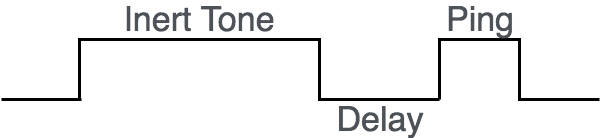
\includegraphics[scale=0.5]{inert_tone}

\caption{An example of a UTP with an ``inert tone'' in place of the first
ping.} \label{fig-inert}
\end{figure}

In this solution, we would still be able to detect collisions because the
pings and delay would have mathematically-determined values, and any collision
could cause one or more of those values to be altered, meaning that they
would no longer be copacetic.

\subsubsection{Benefits}

This method does not require a change to {\em standard} UTP formatting, and
removal of the boolean value encoding requirement would not affect previous
work.

This method is resistant to collisions, so long as the appropriate restrictions
are placed on the duration of each inert tone.

A UTP with an inert tone is clearly distinguishable from a standard UTP.
This means that there is no arbitrarily-defined distinction between standard
and inert UTPs.
For instance, a simple visual inspection of a given UTP could quickly and
easily determine if a UTP came from an inert transmitter or not.

Because the inert tone is considerably longer than most other transmissions,
this method may cause the battery in the transmitter to die sooner.
Since there is no need to repeatedly record the location of a transmitter that
does not move, this may conveniently lead to the inert transmitter ceasing its
transmissions earlier than it otherwise would.
This is speculation and will depend on the actual hardware performance, though,
so it is only a small consideration.

\subsubsection{Drawbacks}

The total duration of a UTP with an inert tone would be considerably longer
than a standard UTP, which means we may have more collisions.

This method will also require additional processing and calculations by the
receiver, though the same may be said of {\em almost} any other alternative.

%\subsubsection{Edge Cases}
%
%If a standard UTP and an inert UTP were broadcast from nearby locations at
%similar enough times, the extra-long inert tone in the later broadcast could
%completely mask the standard UTP.
%However, this is not necessarily a bad thing, as it would mean that a
%collision occurred but that it did not interrupt or affect the transmission
%and decoding of the inert transmitter's signal.

\section{Discussion}

The development team has come to the consensus that option \ref{adj-both-pings}
is the most advisable choice for this project.
The appeal of this method is largely its simplicity:
it requires no additional calculations on the part of the receiver, as it
utilizes the existing encoding scheme that will already be implemented.

The only thing left to determine is how divide the UTP space between the two
values.
The suggestion of this author is to use the first $MAX\_ID$ values exactly as
they otherwise would be used (with the boolean value FALSE)
and to reserve the values in the range $(MAX\_ID,\ 2 \times MAX\_ID]$ for
use when the boolean value is TRUE.
However, {\em this is not a formal definition};
see the official iCRAB Transmission Protocol Definition document for accurate
details.

\end{document}

